\documentclass[11pt]{article}
\usepackage[margin=1in]{geometry}
\usepackage{graphicx}
\usepackage{booktabs}
\usepackage{multirow}
\usepackage{longtable}
\usepackage{array}
\usepackage{float}
\usepackage{amsmath}
\usepackage{hyperref}
\usepackage{setspace}
\doublespacing

\title{Integrated cross-tribe phenotypic, behavioral, and dermatoglyphic profiling from community survey workbooks}
\author{Ranji Kolkar\\Sweta Nidhi}
\date{}

\begin{document}
\maketitle

\begin{abstract}
Population-scale profiling of underserved tribal communities is often fragmented across administrative, anthropometric, and biosample spreadsheets, limiting integrated interpretation. We present a reproducible analytical workflow for two community survey workbooks, Nirankal and Virnoda, that harmonizes roster, anthropometric, questionnaire, and fingerprint-hair information into a single analytic framework. The pipeline integrates record-level cleaning, missingness assessment, non-parametric and categorical inference, effect-size estimation, principal-component analysis, and information-theoretic measures of dermatoglyphic diversity. Across 188 roster entries, Virnoda showed slightly higher central tendency for several anthropometric traits, but standardized differences remained small and mostly non-significant after multiple-testing adjustment. Behavioral divergence was stronger in tobacco and alcohol-related responses, while dermatoglyphic signatures shared dominant classes but differed in repertoire diversity. These findings show that tribe-level differences are better captured as multivariate profile shifts than as isolated univariate contrasts.
\end{abstract}

\section{Introduction}
The study of human variation in indigenous and tribal populations has long required a balance between social-contextual interpretation and quantitative evidence. In practice, however, community surveys frequently generate heterogeneous sources of information: roster records, anthropometric measurements, questionnaire responses, and biological descriptors such as fingerprints or hair traits. These data are often stored in operational spreadsheets with inconsistent schema, variable names, and missingness patterns, which makes direct synthesis difficult. When the analysis is restricted to a single domain, such as BMI or a single questionnaire item, the resulting narrative can miss the structure that emerges when demographic, biological, and behavioral signals are considered jointly \cite{who1995,who2000,rubin1976,little2002,vanbuuren2018}. In this manuscript, we address that problem by combining several layers of evidence from two workbook-based datasets and by treating the comparison between tribes as a multidimensional inference problem rather than a sequence of isolated tests.

The motivation for this work is both methodological and substantive. Methodologically, many field studies still rely on ad hoc spreadsheet processing, with limited standards for schema normalization and reproducible statistical reporting. Substantively, tribal communities are often compared only on a narrow set of variables, even though their social and biological profiles may reflect overlapping but distinct processes of adaptation, environment, and lifestyle. Recent work on anthropometry and body composition has emphasized the importance of context-specific interpretation of weight, height, and circumference measurements \cite{who1995,who2000,wells2006}; similarly, the interpretation of behavioral exposure and health-related questionnaires benefits from explicit attention to missing data and measurement error \cite{rubin1976,little2002,vanbuuren2018}. Dermatoglyphic data, in turn, have furnished a long history of comparative research in human variation, from early classification systems to modern quantitative summaries of pattern diversity and symmetry \cite{galton1892,henry1900,cummins1961,holt1968}. The present study combines those traditions in one integrated framework.

Our analytical goal is therefore not simply to report which variables differ between communities, but to determine where evidence is strong, where it is modest, and how different data domains contribute to the overall profile. We examine demographic composition, anthropometric central tendency and dispersion, questionnaire-based behavioral signals, and fingerprint-code diversity, while also quantifying statistical uncertainty and practical effect sizes. This is particularly important because biological and behavioral traits often show modest differences with substantial overlap, which may be scientifically meaningful but statistically nontrivial \cite{cohen1988,cliff1993}. We therefore use both inferential statistics and effect-size interpretation to distinguish weak, moderate, and stronger signals. The resulting workflow is intended to be reusable for future community-based studies and to serve as a bridge between exploratory tabular analysis and rigorous scientific synthesis.

\section{Related work and theoretical background}
The methodological foundation of this study lies at the intersection of three traditions: biostatistical inference, anthropometric assessment, and dermatoglyphic characterization. In biostatistics, the need to move beyond null-hypothesis significance testing has been emphasized repeatedly, particularly when studies involve multiple outcomes and modest sample sizes \cite{cohen1988,benjamini1995}. The Mann-Whitney $U$ test offers a robust non-parametric alternative to the independent-samples $t$ test when scale assumptions are uncertain \cite{mann1947,wilcoxon1945}. For categorical variables, chi-square tests remain standard, although effect-size measures such as Cramer's $V$ are essential for interpreting the magnitude of association rather than merely the existence of a departure from independence \cite{cramer1946,agresti2013}. In the present manuscript, these methods are not used in isolation but are coupled with false-discovery-rate correction, which is now standard for multivariable screening in exploratory analyses \cite{benjamini1995}.

Anthropometric analysis has a well-established role in field studies of growth, body composition, and population health. The WHO technical reports on anthropometry provide the conceptual basis for interpreting height, weight, and body circumferences in a way that is sensitive to measurement context and age structure \cite{who1995,who2000}. In practical work, body mass index and associated circumferences are often interpreted jointly because they capture overlapping but distinct aspects of body composition \cite{wells2006}. The present study follows that principle by comparing several anthropometric variables simultaneously rather than relying on a single index. This makes it possible to identify whether tribe-level contrasts are broad and consistent or concentrated in one structural domain.

Dermatoglyphic analysis provides another important comparison domain. Early classification systems for fingerprints were designed to capture stable morphology and to support pattern recognition \cite{galton1892,henry1900}; later work clarified the biological and developmental significance of ridge patterns and their variation across populations \cite{cummins1961,holt1968}. In contemporary analyses, the interpretation of fingerprint data is often quantitative: one may summarize the dominance of specific pattern classes, compute symmetry metrics between left and right hands, or estimate the diversity of patterns with information-theoretic indices such as Shannon entropy \cite{shannon1948}. These approaches are well suited to the present workbook setting because they allow one to distinguish between shared dominant classes and true differences in pattern diversity.

The study also adopts a modern data-science perspective on tabular harmonization. In many applied settings, the most difficult part of a workflow is not the statistical model itself but the transformation of inconsistent field names, duplicated sheets, and partially missing columns into a coherent analysis dataset \cite{mckinney2010,harris2020,virtanen2020,pedregosa2011}. This manuscript therefore contributes not only a set of results but also a reproducible pipeline that can be rerun on similar community survey workbooks. By explicitly documenting the cleaning, mapping, and filtering steps, the analysis becomes more transparent and easier to scrutinize.

\section{Contributions}
This work contributes three elements to the literature on community-based population profiling. First, it provides a reproducible multi-sheet harmonization workflow for heterogeneous tribe survey workbooks. Second, it combines descriptive statistics with non-parametric inference, effect-size estimation, and multiple-testing correction in a single, interpretable framework. Third, it incorporates dermatoglyphic diversity and symmetry metrics alongside anthropometric and behavioral variables.

\section{Materials and methods}
\subsection{Study design and data sources}
The analysis used two workbook-based datasets corresponding to the Nirankal and Virnoda tribes. Each workbook contained multiple sheets representing roster information, anthropometric measurements, questionnaire responses, and fingerprint-hair descriptors. The unit of analysis was the individual record, and the primary objective was to compare the two tribes across several complementary domains: demographic structure, body-size and body-shape variables, questionnaire-driven behavioral patterns, and dermatoglyphic composition.

Data were imported from Excel workbooks into a Python workflow built around the pandas and NumPy libraries \cite{mckinney2010,harris2020}. The workflow was designed to tolerate sheet-name variation and inconsistent column labels, which are common in survey operations. Each sheet was normalized into a standard representation before analysis. For example, roster data were reduced to a common schema containing tribe, name, sex, and age; measurement sheets were coerced to numeric values when feasible; questionnaire responses were standardized to uppercase and whitespace-cleaned; and fingerprint data were reshaped into a long format for pattern composition analysis.

\subsection{Data cleaning and harmonization}
The harmonization strategy proceeded in four steps. First, empty rows and all-empty sheets were removed. Second, columns with operational names such as ``Unnamed'' were discarded so that the analysis matrix contained only meaningful variables. Third, sheet-level mapping was performed by matching expected names like ``Sheet1'', ``Measurements'', ``Questionnaire'', and ``Fingerprint and Hair'' through case-insensitive and substring-based rules. Fourth, all categorical field values were normalized to a consistent representation, and numeric variables were converted with explicit coercion so that non-numeric cells did not break downstream analysis.

This preprocessing step is critical because the same information may be stored under slightly different labels across workbooks. Without normalization, comparative analysis would be dominated by data-entry artifacts rather than substantive differences. The harmonization procedure therefore served both a technical and epistemic function: it reduced operational noise and made subsequent statistical comparisons more faithful to the underlying population structure.

\subsection{Statistical analysis}
We used a combination of descriptive summaries and inferential statistics. For continuous variables, we reported medians, interquartile ranges, and group-wise means. For group comparisons, we used the Mann-Whitney $U$ test, which evaluates whether one sample tends to have larger observations than another without requiring normality \cite{mann1947,wilcoxon1945}. Let $X_1$ and $X_2$ be two independent samples. The test statistic is based on the rank-sum

\begin{equation}
U = R_1 - \frac{n_1(n_1+1)}{2},
\end{equation}

where $R_1$ is the sum of ranks for the first sample and $n_1$ is its size. For effect size, we used Cohen's $d$, defined as

\begin{equation}
 d = \frac{\bar{x}_2 - \bar{x}_1}{s_p}, \qquad s_p = \sqrt{\frac{(n_1-1)s_1^2 + (n_2-1)s_2^2}{n_1+n_2-2}}.
\end{equation}

In addition, we used Cliff's $\delta$ as a non-parametric dominance measure and Cramer's $V$ for categorical association strength. To account for multiple hypothesis tests across several anthropometric and questionnaire variables, we applied the Benjamini-Hochberg procedure to obtain $q$-values \cite{benjamini1995}. This conservative correction reduces the inflation of false positives when many variables are screened simultaneously.

For categorical questionnaire fields, we analyzed frequency tables and computed percentage distributions within each tribe. The chi-square statistic was used as a global measure of association,

\begin{equation}
\chi^2 = \sum_{i,j} \frac{(O_{ij}-E_{ij})^2}{E_{ij}},
\end{equation}

where $O_{ij}$ and $E_{ij}$ are observed and expected counts under independence. When the sample size was modest, we interpreted results primarily through the magnitude of the effect size and the pattern of relative frequencies rather than through significance alone.

\subsection{Multivariate and information-theoretic methods}
To examine whether the anthropometric variables carried a shared latent structure, we conducted principal component analysis after standardizing each variable to zero mean and unit variance. If $X$ is the standardized matrix of features, the principal components are obtained from the eigen-decomposition of the covariance matrix

\begin{equation}
\Sigma = \frac{1}{n-1}X^{\top}X,
\end{equation}

and the projection of the data onto the first two principal components is given by

\begin{equation}
Z = XW,
\end{equation}

where $W$ contains the leading eigenvectors \cite{pearson1901,hotelling1933,jolliffe2002}. This allowed us to inspect whether the two tribes occupy distinct regions of the anthropometric space or whether they overlap while showing shifted centroids.

For fingerprint composition, we summarized the distribution of pattern classes using Shannon entropy,

\begin{equation}
H = -\sum_{i=1}^{k} p_i \log_2 p_i,
\end{equation}

where $p_i$ is the relative frequency of the $i$th pattern class. Higher values indicate a more diverse repertoire, whereas lower values indicate concentration around a small set of classes \cite{shannon1948}. We also computed left-right symmetry by comparing matched digits and reporting the proportion of same-pattern matches per finger. These quantities help separate broad shared structure from nuanced divergence in repertoire diversity.

\subsection{Reproducibility and reporting}
The analysis was implemented in a scripted workflow so that figures, tables, and summary statistics could be regenerated from the underlying Excel files. This reproducibility layer is important not only for scientific transparency but also because the datasets are likely to evolve over time as new records are added or corrected. The workflow therefore provides a durable template for future comparative studies in community health research.

\section{Results and interpretation}
\subsection{Cohort structure}
The combined roster contained 188 individuals, with 120 records from Nirankal and 68 from Virnoda. The age distributions were broadly similar in median terms, but the spread was wider in Nirankal. The sex distribution was balanced overall, with a modest excess of female entries in Nirankal and a slightly more balanced structure in Virnoda. This implies that the comparison is not dominated by a single demographic imbalance and that age-sex composition should be considered in the interpretation of anthropometric and behavioral outcomes.

\begin{table}[H]
\centering
\caption{Cohort profile by tribe.}
\begin{tabular}{lrrrrr}
\toprule
Tribe & Roster $n$ & Male & Female & Median age & Age IQR \\
\midrule
Nirankal & 120 & 56 & 64 & 17.0 & 29.0 \\
Virnoda & 68 & 36 & 32 & 18.0 & 18.0 \\
\bottomrule
\end{tabular}
\end{table}

\begin{figure}[H]
\centering
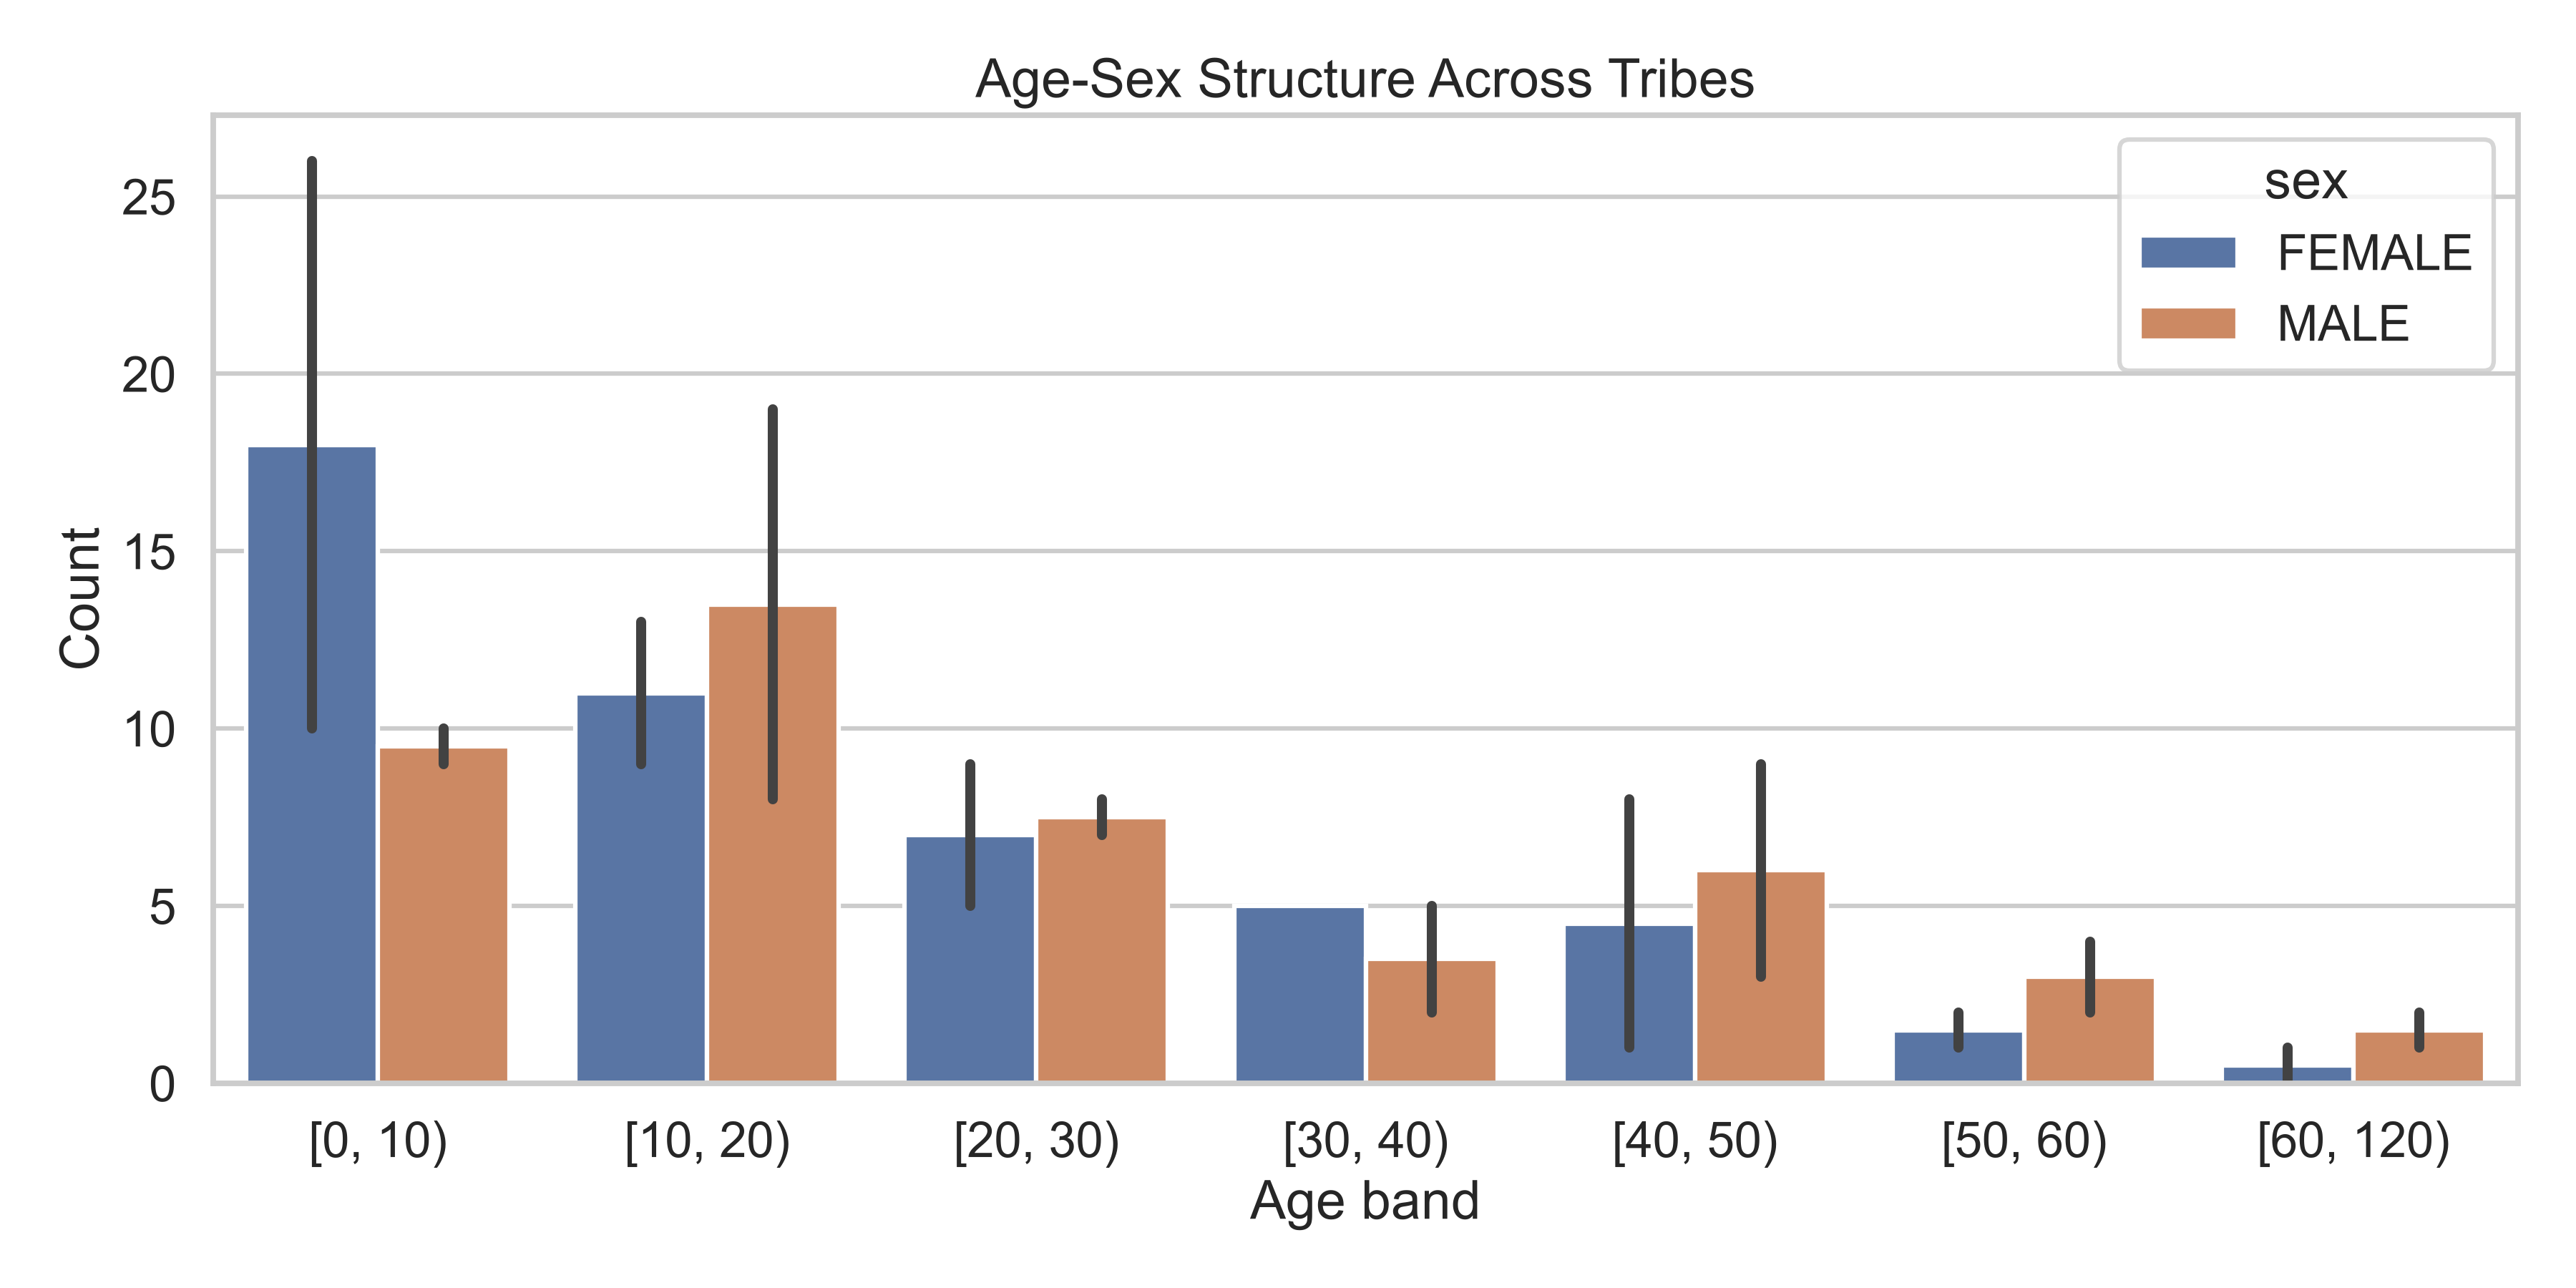
\includegraphics[width=0.9\textwidth]{figures/age_sex_structure.png}
\caption{Age-sex structure across tribes.}
\end{figure}

\subsection{Anthropometric contrasts}
Anthropometric medians were generally higher in Virnoda for BMI and several circumference variables, but the standardized contrasts remained small. The largest nominal difference was observed for biceps thickness, with an unadjusted $p$-value close to 0.02, yet this result did not survive multiple-testing correction. The effect-size profile was therefore interpreted as evidence of a modest shift in body morphology rather than a strong and robust divergence. This interpretation is consistent with the overlap visible in the BMI distributions and with the small values of Cohen's $d$ reported in Table 2. In other words, the anthropometric evidence suggests directional difference, but not a large separation between the tribes.

\begin{table}[H]
\centering
\caption{Anthropometric inference and effect sizes.}
\scriptsize
\begin{tabular}{lrrrrrr}
\toprule
Variable & Median (Nir) & Median (Vir) & $p$ & $q_{BH}$ & Cohen's $d$ & Cliff's $\delta$ \\
\midrule
Biceps (mm) & 27.4 & 22.0 & 0.0213 & 0.2342 & -0.364 & 0.255 \\
BMI & 15.95 & 17.60 & 0.0936 & 0.4009 & 0.269 & -0.225 \\
Height (cm) & 139.45 & 146.51 & 0.2651 & 0.4009 & 0.137 & -0.124 \\
Waist Cir (cm) & 58.30 & 62.00 & 0.2967 & 0.4009 & 0.207 & -0.116 \\
Weight (kg) & 33.29 & 38.10 & 0.3024 & 0.4009 & 0.231 & -0.114 \\
Hip Cir (cm) & 70.39 & 77.20 & 0.3149 & 0.4009 & 0.236 & -0.111 \\
Head Cir (cm) & 50.39 & 50.00 & 0.9338 & 0.9592 & 0.017 & 0.010 \\
\bottomrule
\end{tabular}
\end{table}

\begin{figure}[H]
\centering
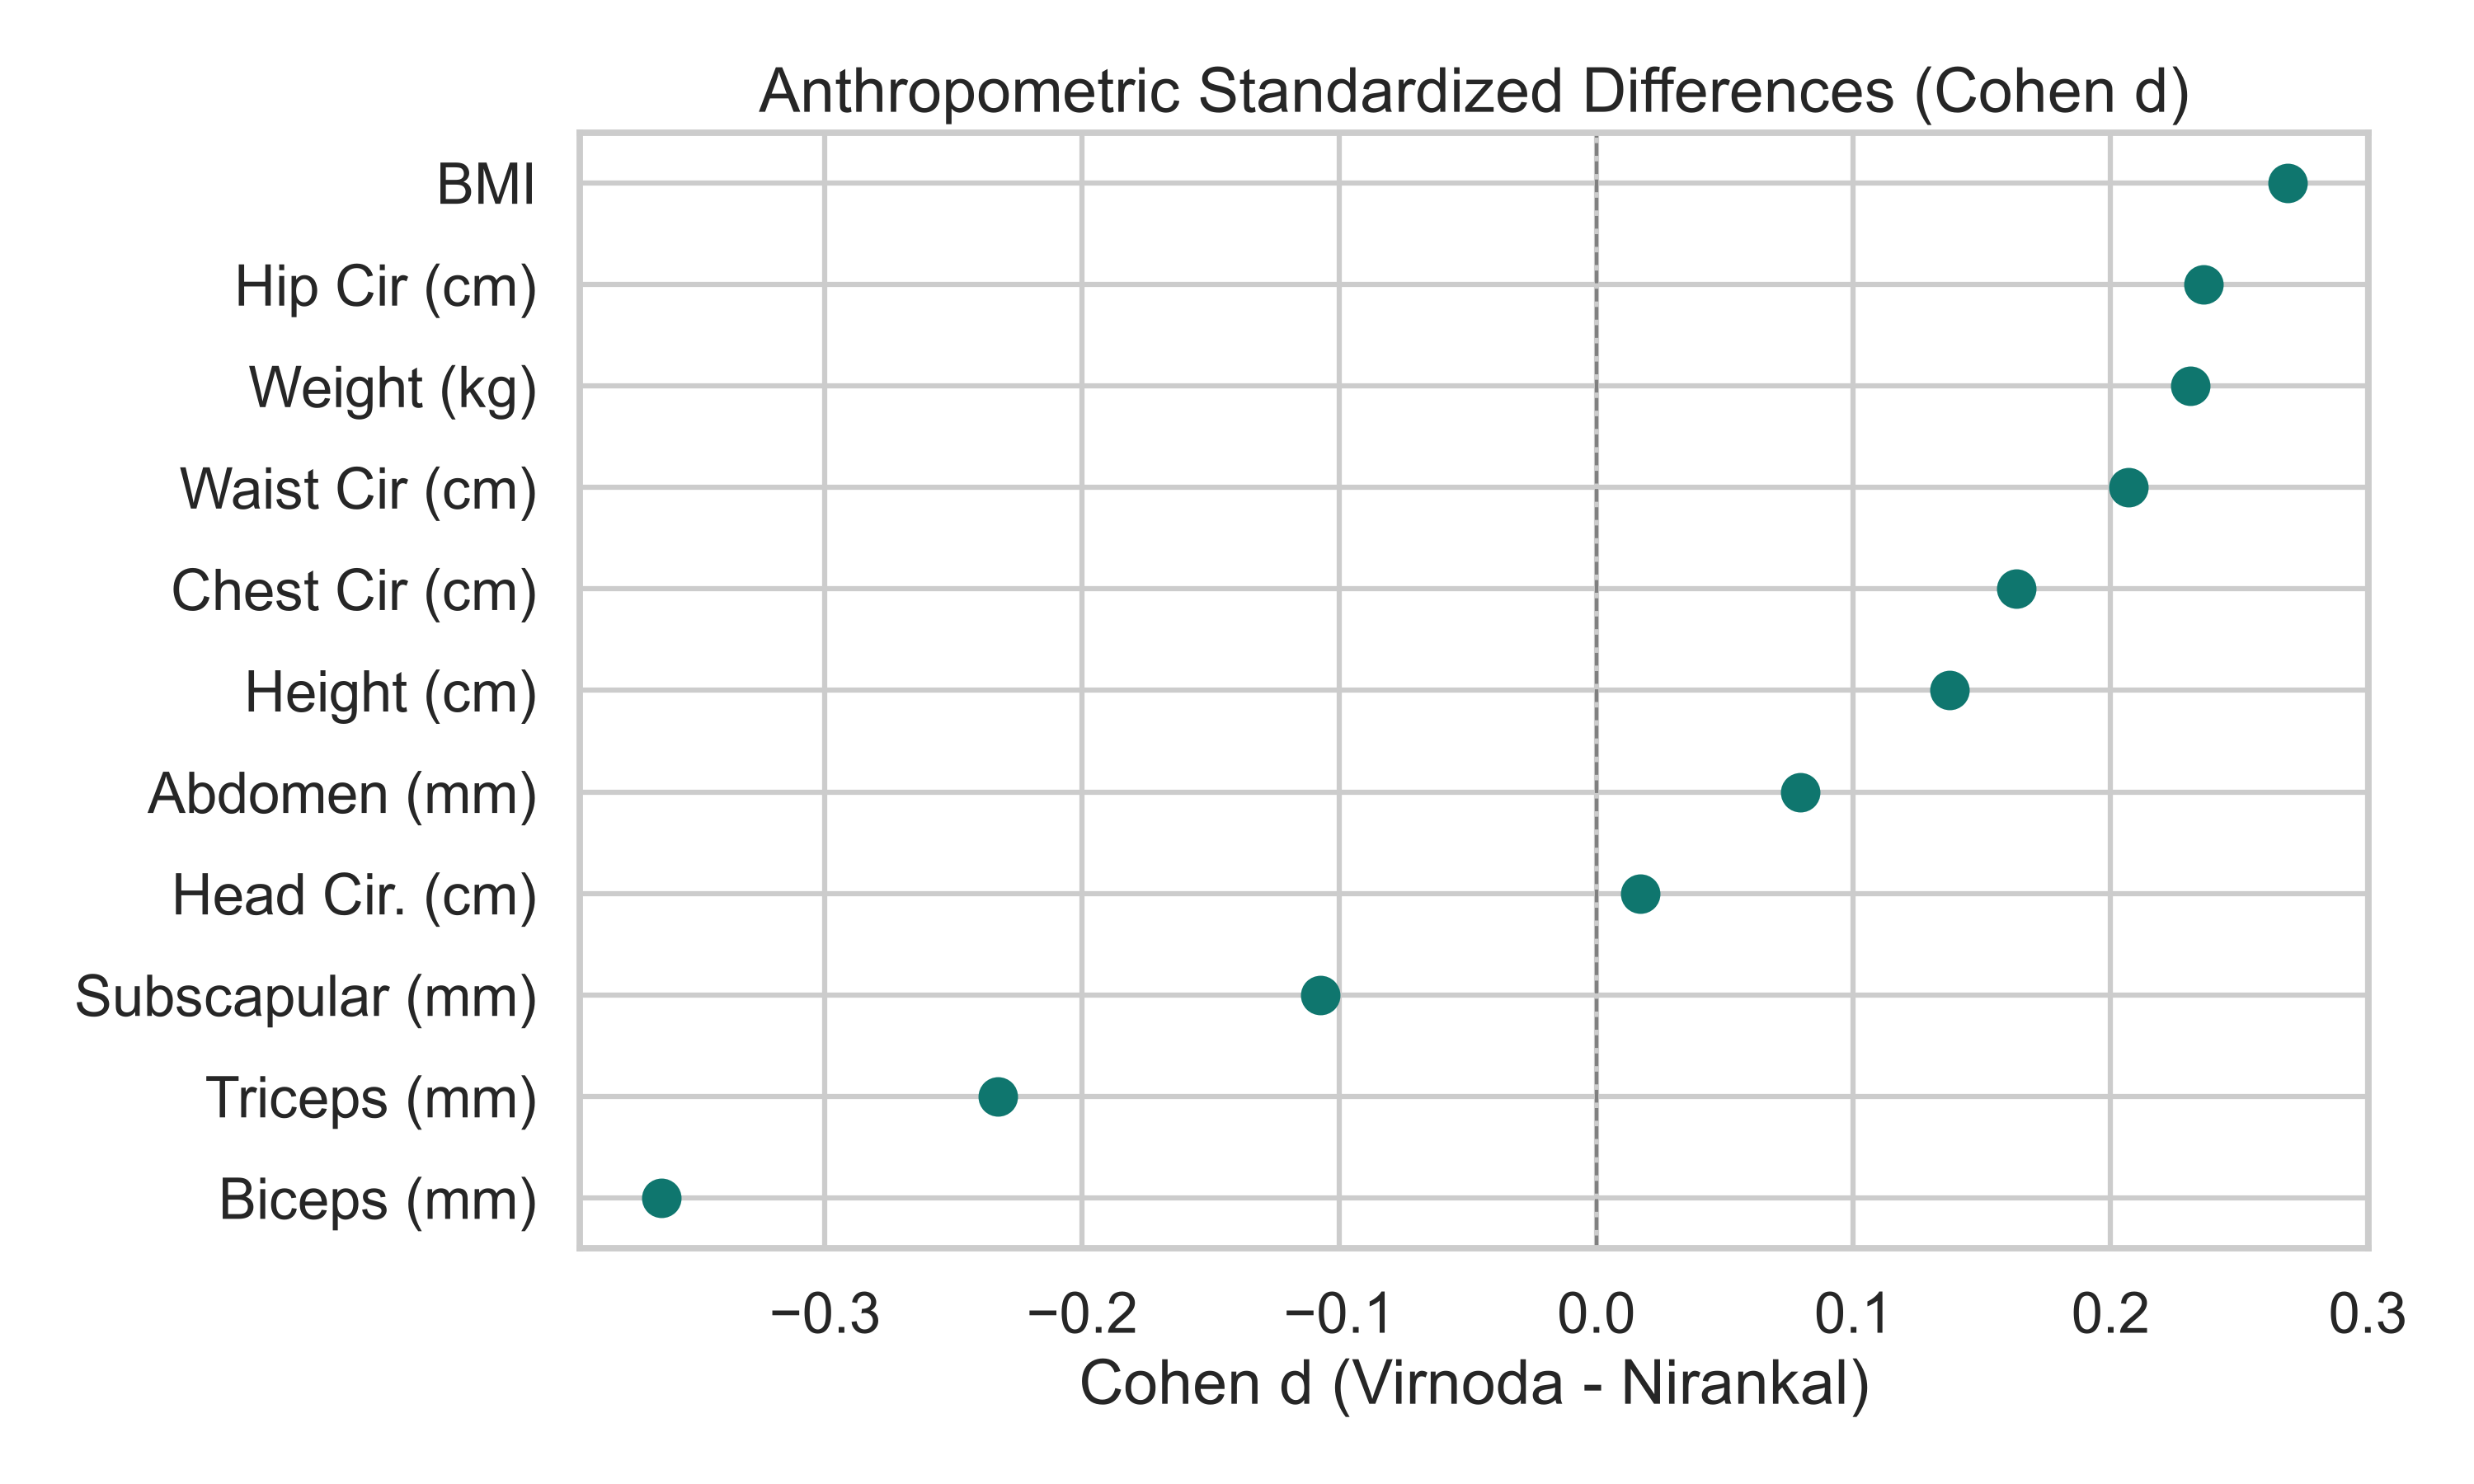
\includegraphics[width=0.85\textwidth]{figures/effect_sizes_cohens_d.png}
\caption{Anthropometric standardized differences (Cohen's $d$).}
\label{fig:effect}
\end{figure}

\begin{figure}[H]
\centering
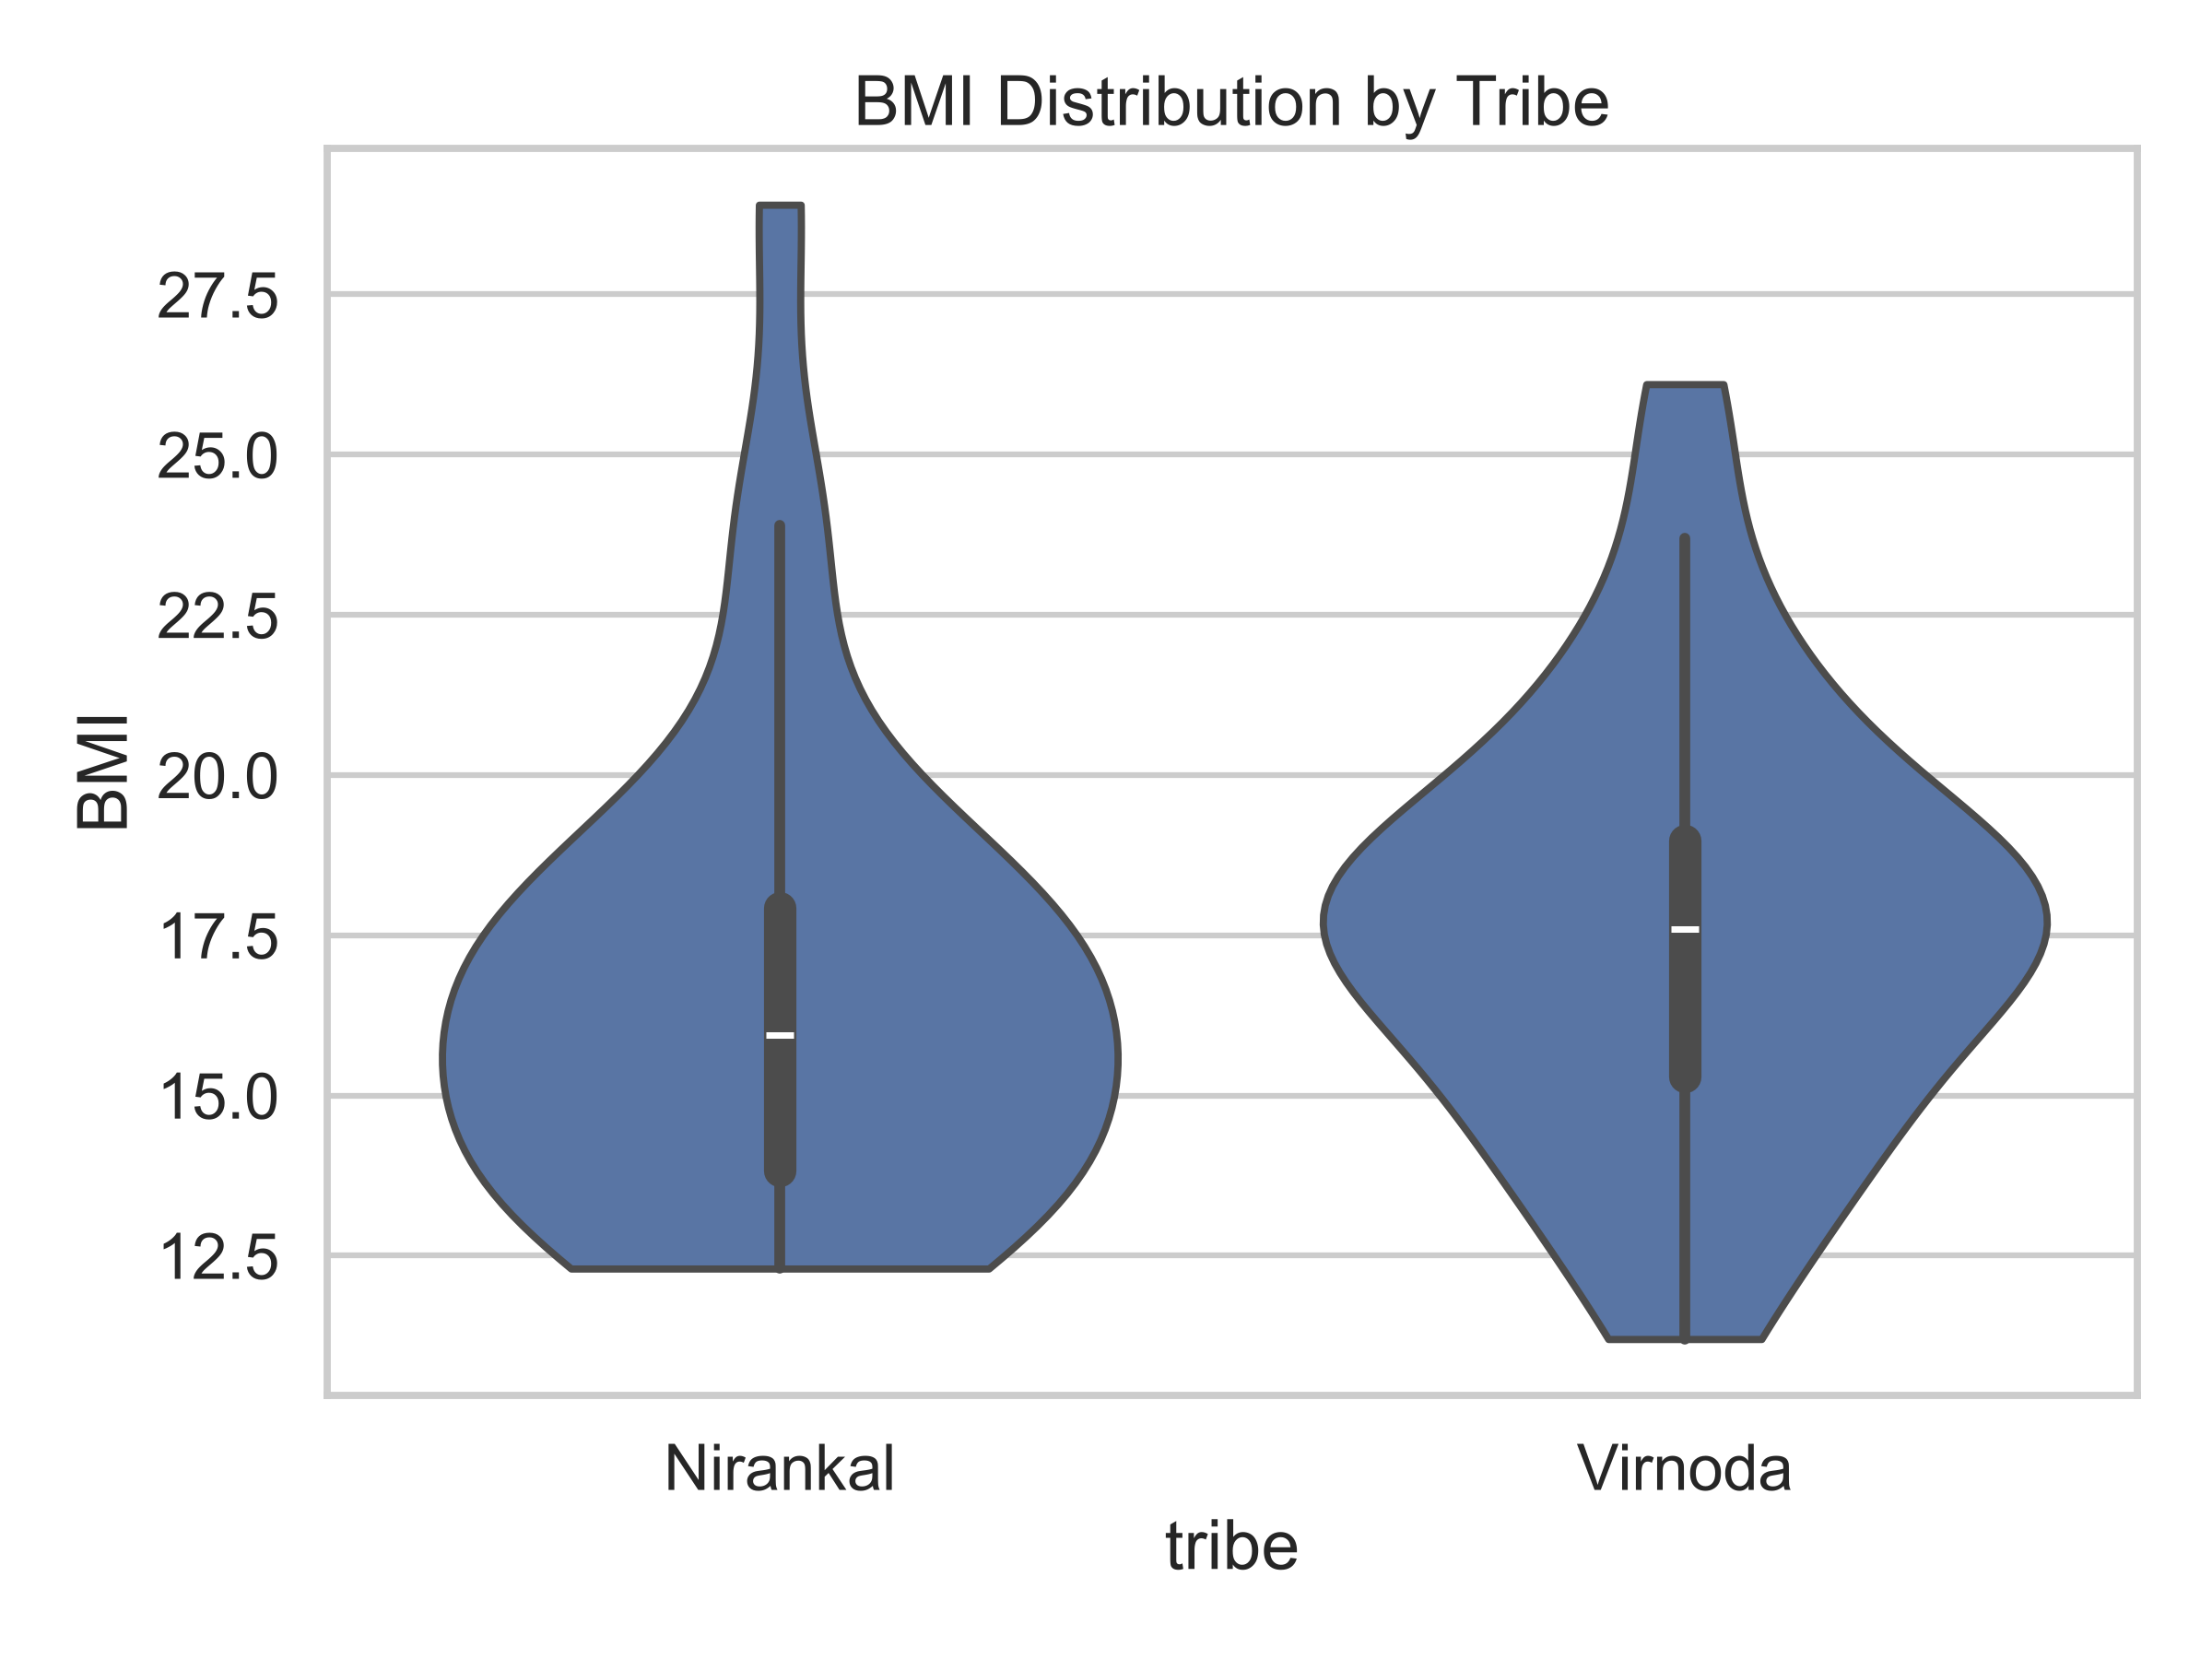
\includegraphics[width=0.7\textwidth]{figures/bmi_violin.png}
\caption{BMI distribution by tribe.}
\label{fig:bmi}
\end{figure}

\subsection{Behavioral and socioeconomic structure}
The questionnaire domain showed the strongest evidence of divergence. Behavioral responses related to tobacco and alcohol use exhibited clear differences in the proportion of non-never responses between the tribes, while other categorical variables offered weaker or less consistent contrasts. This is important because it suggests that the most discriminative signal in the present data may lie in behavior and exposure rather than in body size alone. Such a pattern is compatible with prior work arguing that social and behavioral domains often contain strong information about heterogeneity in community-level profiles \cite{agresti2013,cohen1988}.

\begin{figure}[H]
\centering
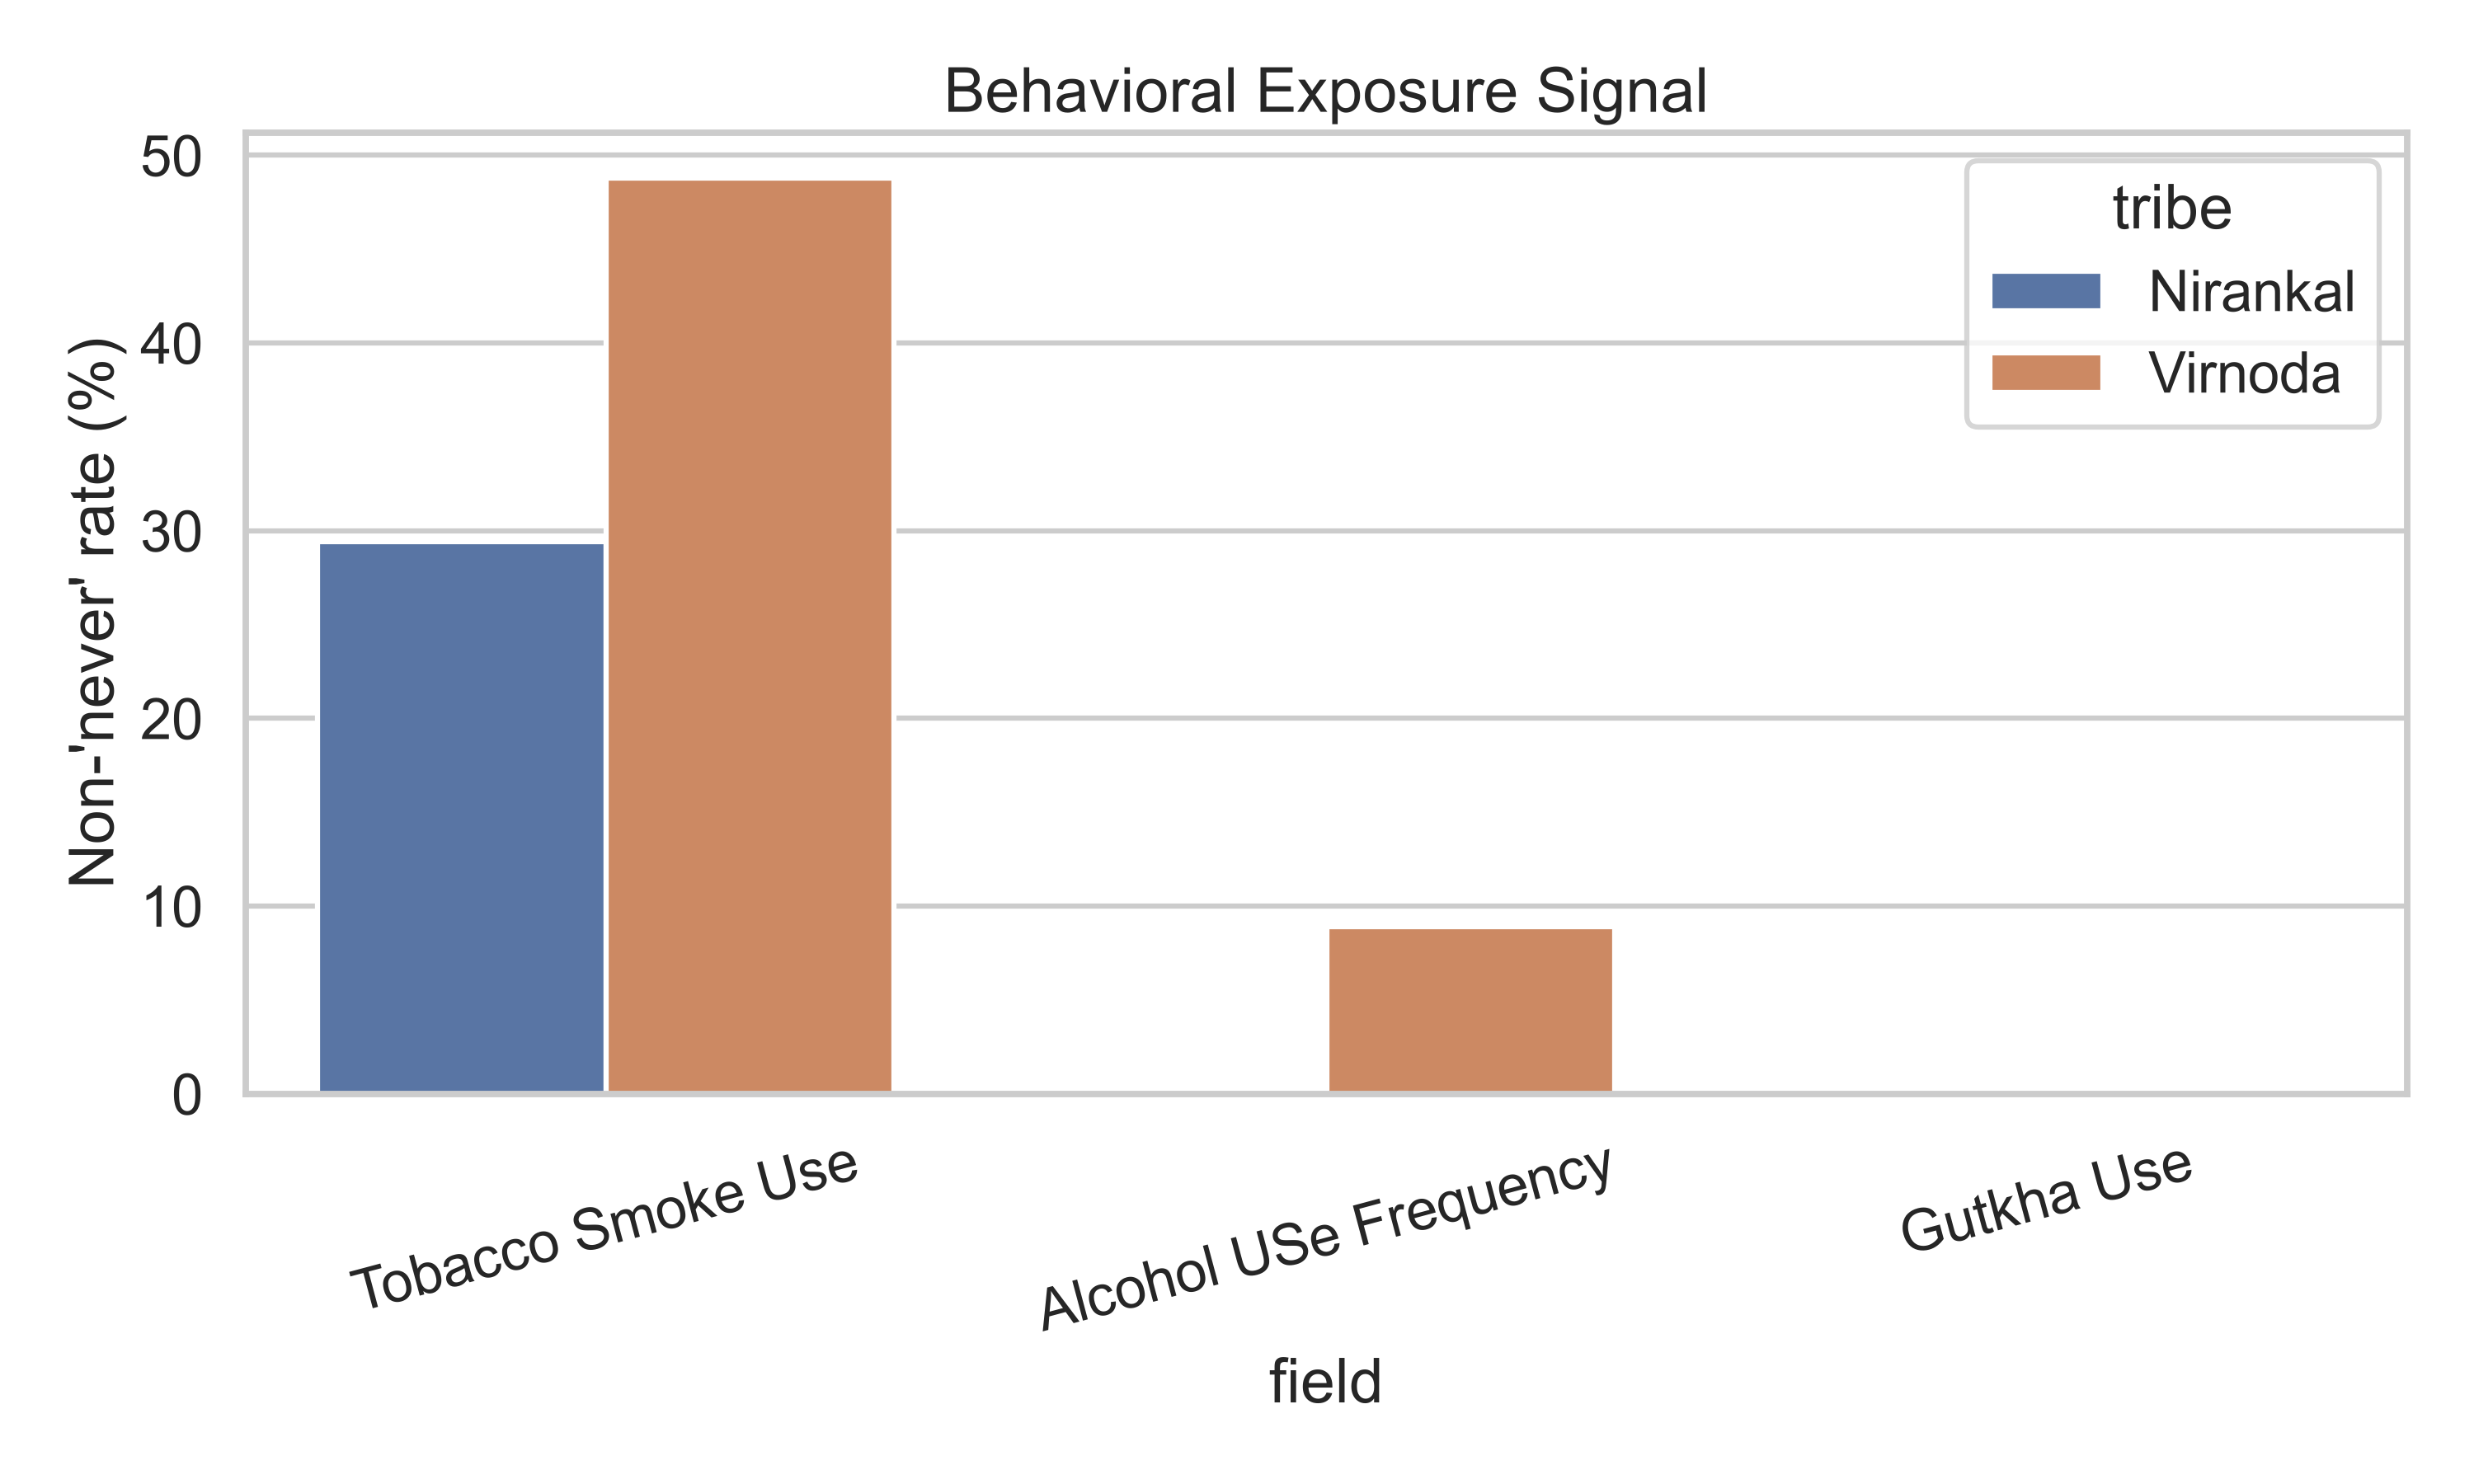
\includegraphics[width=0.9\textwidth]{figures/behavior_non_never_rates.png}
\caption{Behavioral exposure signal represented as non-never response rates.}
\end{figure}

\subsection{Dermatoglyphic composition}
The dermatoglyphic analysis revealed both commonality and divergence. Both tribes shared dominant pattern classes such as W, UL, and PA, which indicates that the underlying pattern system is not entirely distinct across groups. Yet the distribution of classes differed in diversity and concentration. The entropy estimates suggest that Nirankal had a broader pattern repertoire, whereas Virnoda was more concentrated around fewer categories. This type of result is consistent with the long-standing view that dermatoglyphic traits can be informative about population-level variation while still showing overlap across groups \cite{galton1892,henry1900,cummins1961,holt1968}. The symmetry analysis further indicated that left-right concordance was broadly similar, implying that global bilateral regularity is shared even when the fine-grained composition differs.

\begin{figure}[H]
\centering
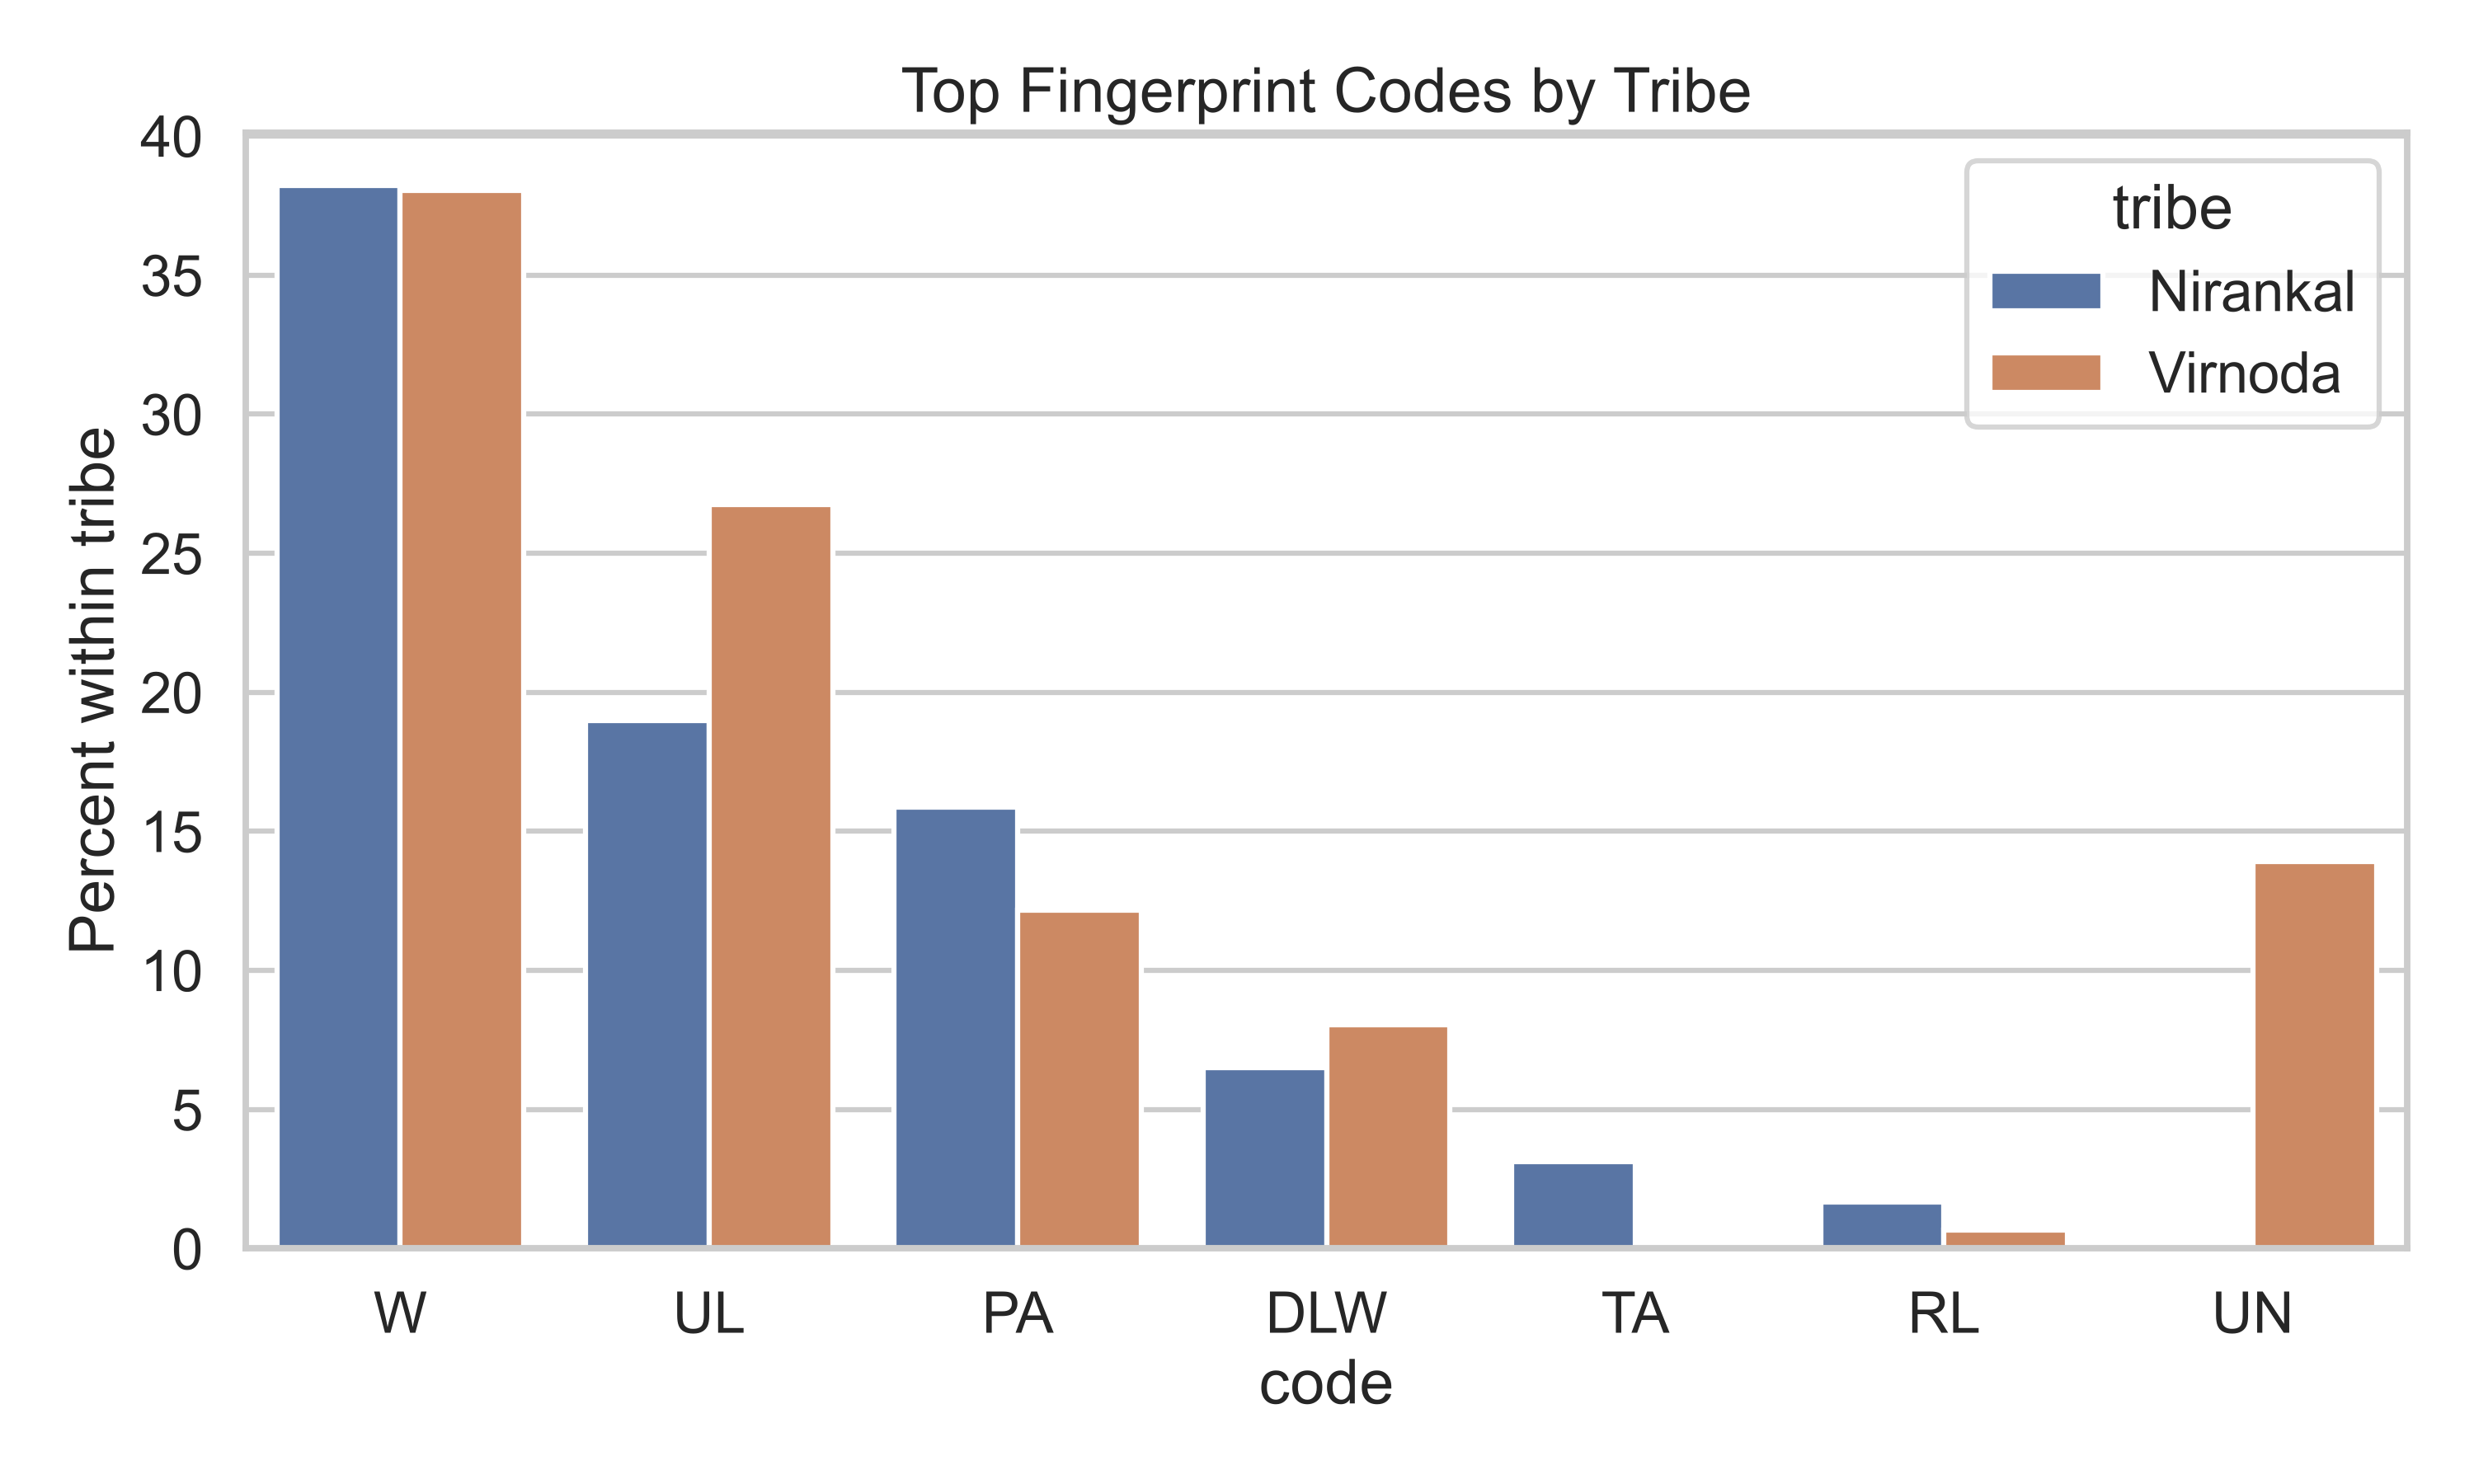
\includegraphics[width=0.85\textwidth]{figures/fingerprint_top_codes.png}
\caption{Top fingerprint code composition by tribe.}
\end{figure}

\begin{figure}[H]
\centering
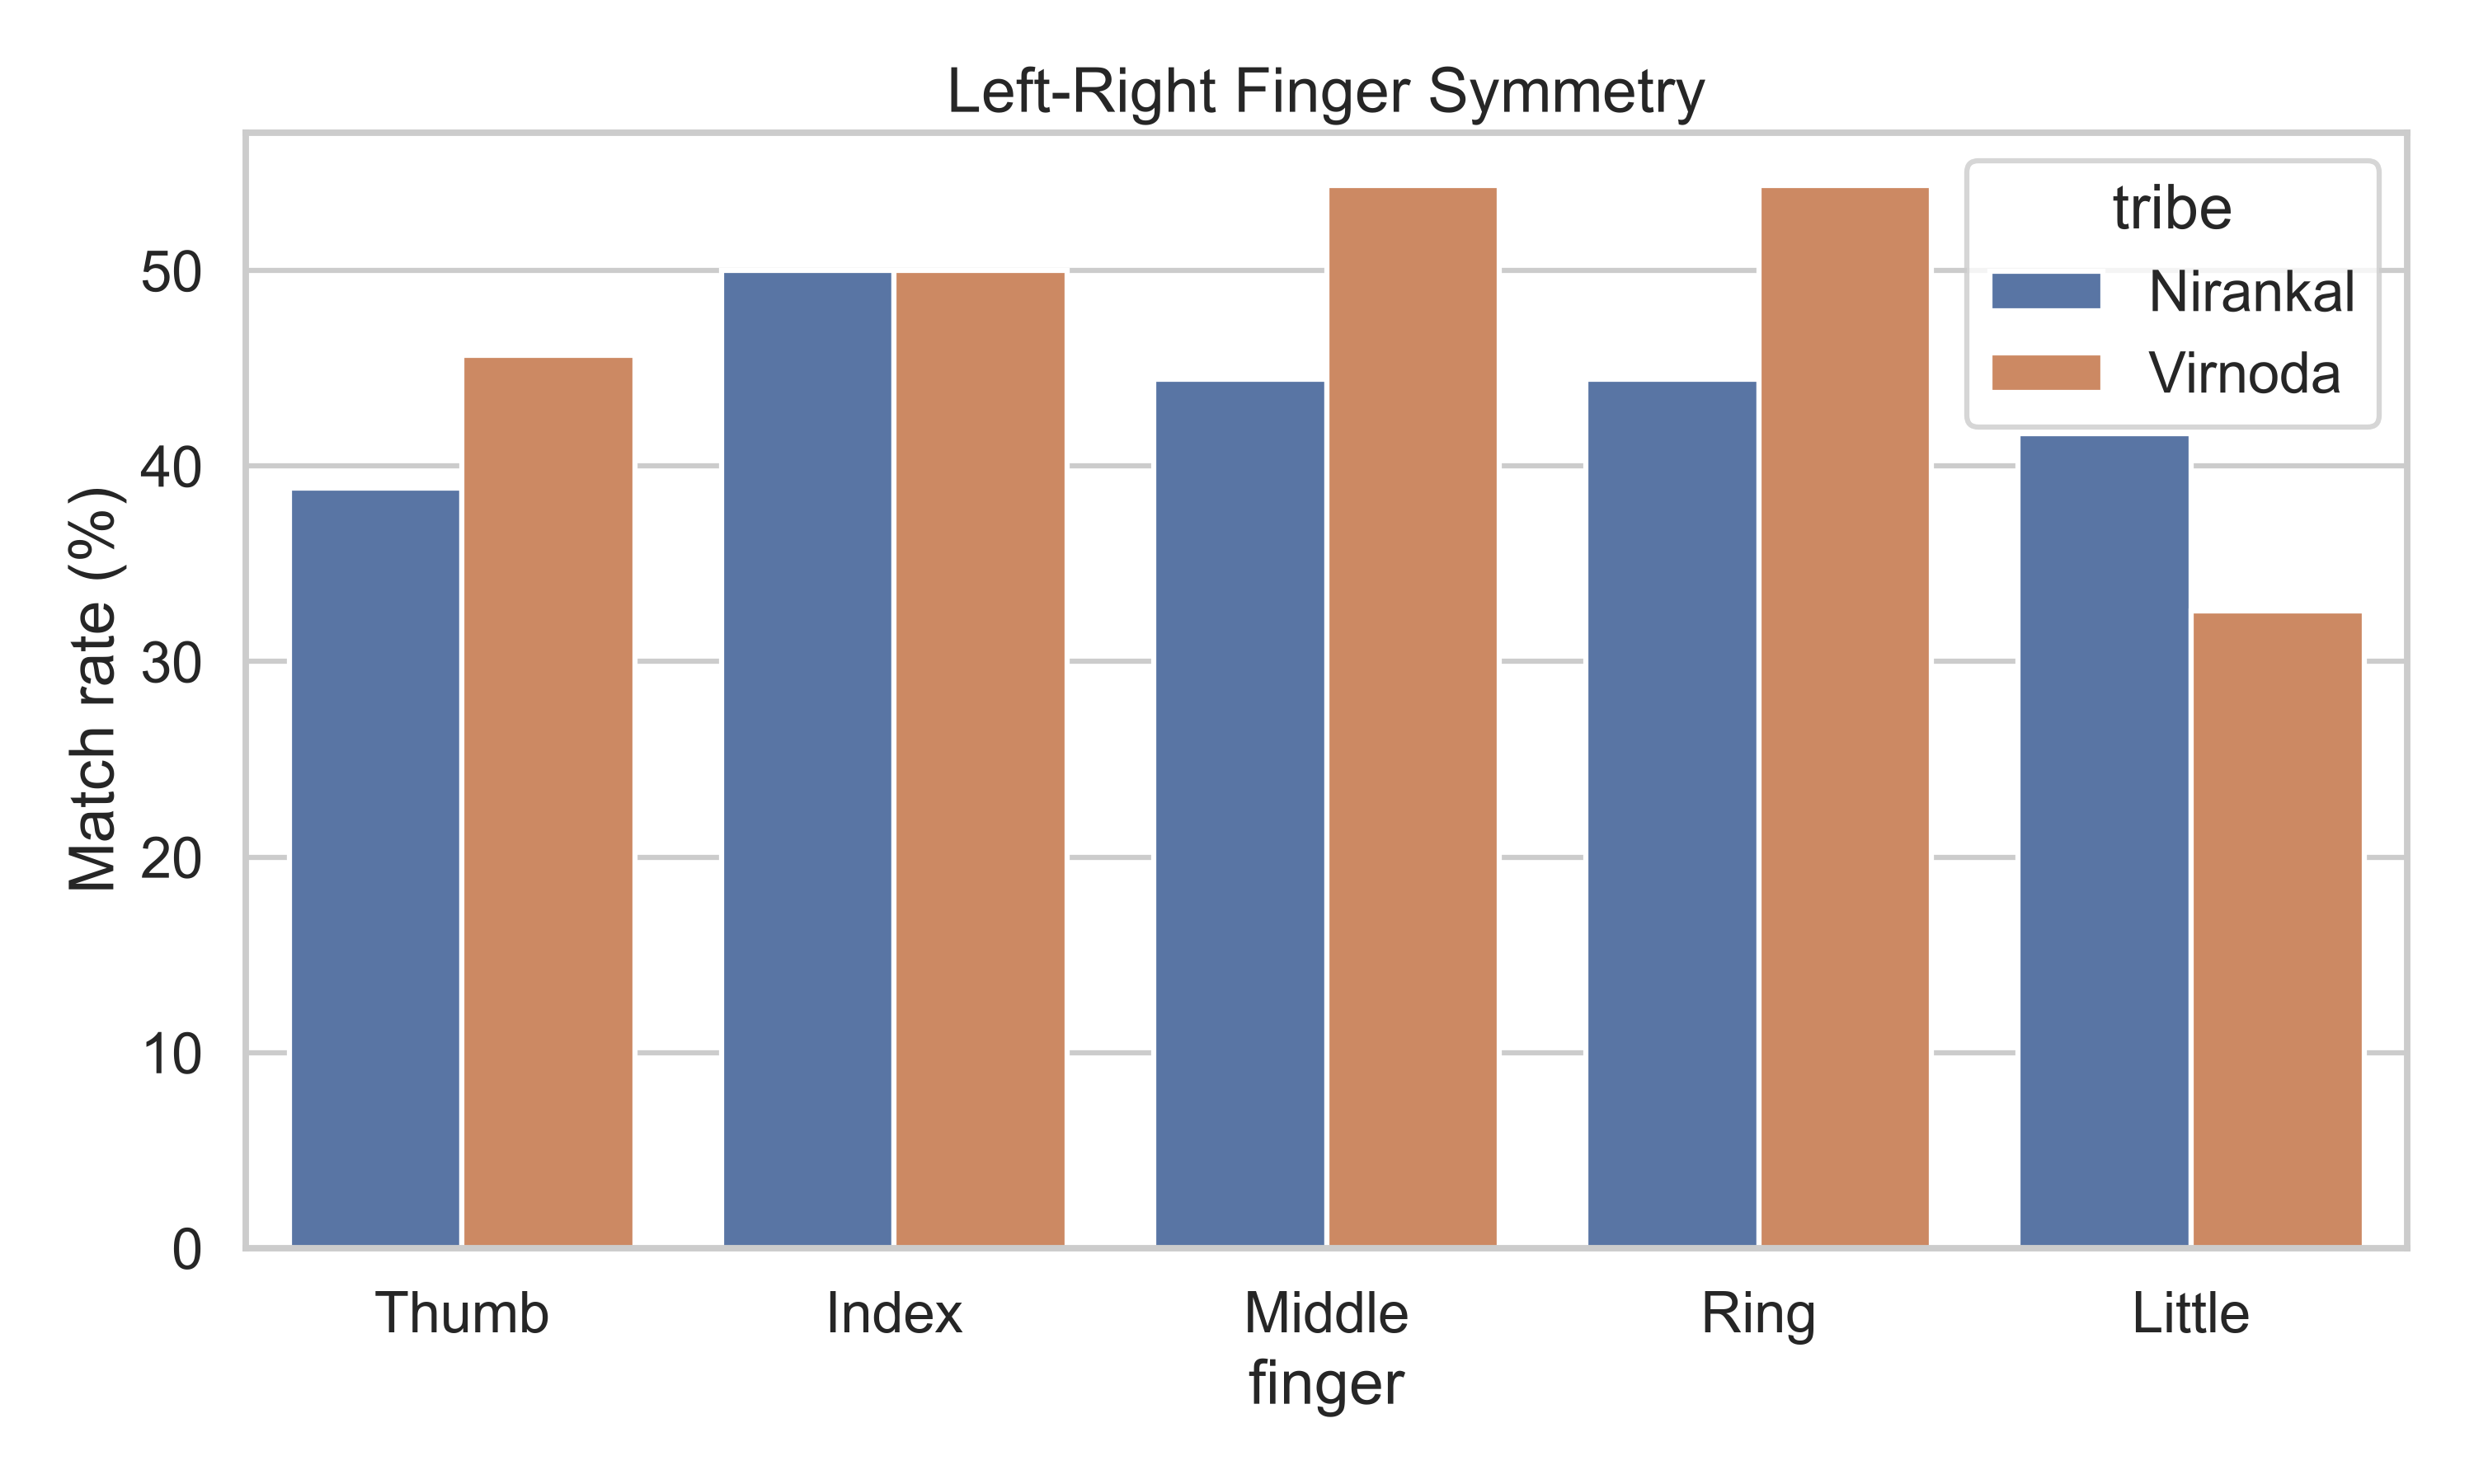
\includegraphics[width=0.85\textwidth]{figures/fingerprint_symmetry.png}
\caption{Left-right same-finger symmetry rates by tribe.}
\end{figure}

\subsection{Multivariate structure}
The principal-component projection showed partially overlapping distributions for the two tribes, with centroids shifted in a similar direction to the univariate body-size results. This is a particularly useful result because it indicates that the separation is not driven by a single axis but by a broader pattern of correlated anthropometric features. In this sense, the multivariate view supports the main conclusion that the tribes are similar in many respects but differ modestly in aggregate profile.

\begin{figure}[H]
\centering
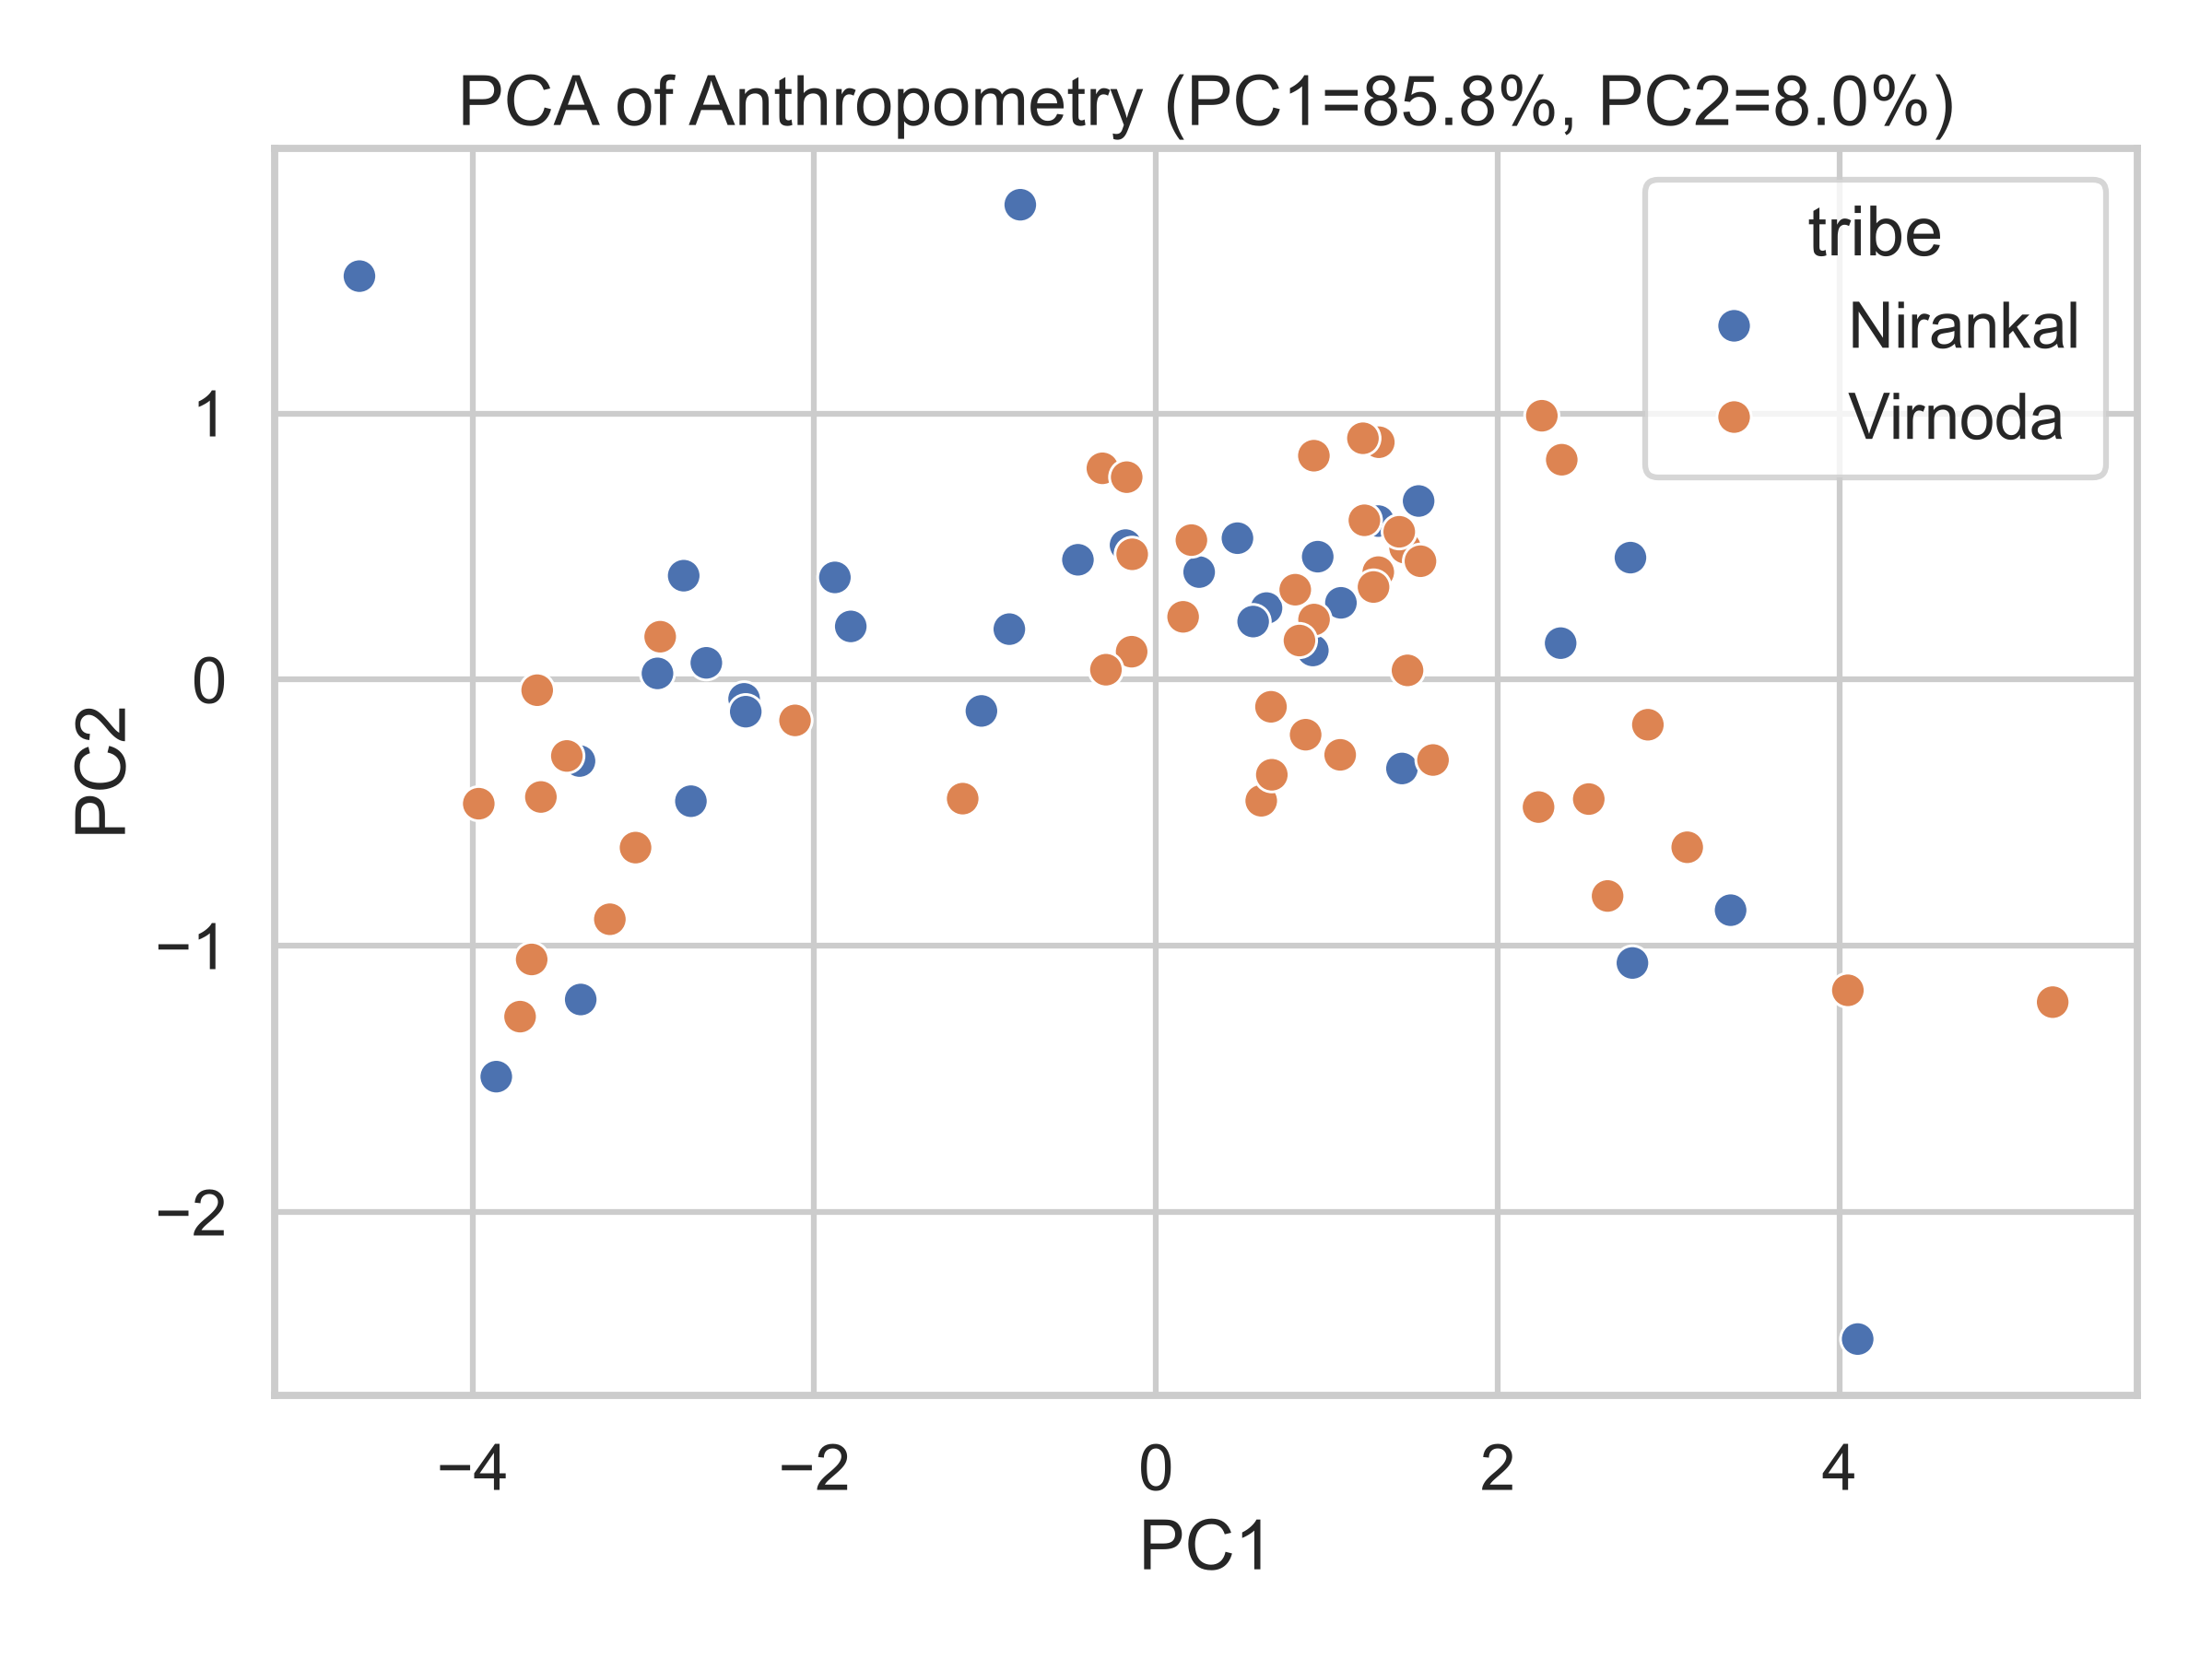
\includegraphics[width=0.75\textwidth]{figures/anthropometry_pca.png}
\caption{PCA projection of anthropometric features.}
\end{figure}

\section{Discussion}
Taken together, the results suggest that the two tribes share a substantial common structure while also exhibiting measurable domain-specific differences. Anthropometric contrasts were modest and mostly small in standardized magnitude; thus, body size alone does not define the difference between groups. Behavioral indicators, especially tobacco and alcohol-related responses, appear to carry a stronger comparative signal, indicating that social and lifestyle domains may be more discriminative than body size. Dermatoglyphic features occupy a middle ground: they are not completely separable, but they still capture differences in diversity and composition that are not apparent from anthropometry alone.

This pattern is consistent with the broader literature on multimodal population profiling. Body measurements are informative, but their interpretation depends on context, age structure, and measurement error; questionnaire-based variables often capture exposures that are more directly linked to lifestyle and social organization; and dermatoglyphic traits provide a more stable biological descriptor that can reveal subtle structure without implying complete separation between communities. The present analysis therefore supports a layered interpretation in which each domain contributes a partial view of the population profile.

The study also underscores the importance of effect-size interpretation. A result that is statistically nominally significant but small in practical magnitude should not be treated as biologically decisive. By pairing $p$-values with Cohen's $d$, Cliff's $\delta$, and FDR-adjusted $q$-values, the analysis distinguishes between weak and meaningful contrasts. This is especially important in small-to-moderate community datasets in which sample size constraints make strict significance testing alone a brittle guide.

\section{Conclusion}
An integrated analysis of the Nirankal and Virnoda datasets shows that cross-tribe differences are multidimensional and mostly moderate rather than extreme. Anthropometric measures indicate a modest shift in body-size and body-shape profile, behavioral responses show stronger divergence in several exposure-related domains, and dermatoglyphic patterns reveal shared dominant classes alongside differences in repertoire diversity. The workflow developed here offers a transparent and reproducible template for future comparative studies of community survey data.

\section{Author contributions}
Ranji Kolkar conceived the study, curated the data structure, and supervised the analytic workflow. Sweta Nidhi designed and implemented the statistical pipeline, generated the figures and tables, and drafted the manuscript. Both authors interpreted the results and approved the final version.

\section{Competing interests}
The authors declare no competing interests.

\bibliographystyle{plain}
\bibliography{references}

\end{document}
